\documentclass{article}

\usepackage{graphicx}
\usepackage{tikz}
\usepackage{tikzsymbols}
\usetikzlibrary{calc,patterns,shapes.geometric}
\pagestyle{empty}
\usepackage[margin=0pt]{geometry}
\geometry{papersize={14in,12in}}

\def\centerarc[#1](#2)(#3:#4:#5){\draw[#1] ($(#2)+({#5*cos(#3)},{#5*sin(#3)})$) arc (#3:#4:#5);}

\begin{document}
	\begin{figure}
		\centering
		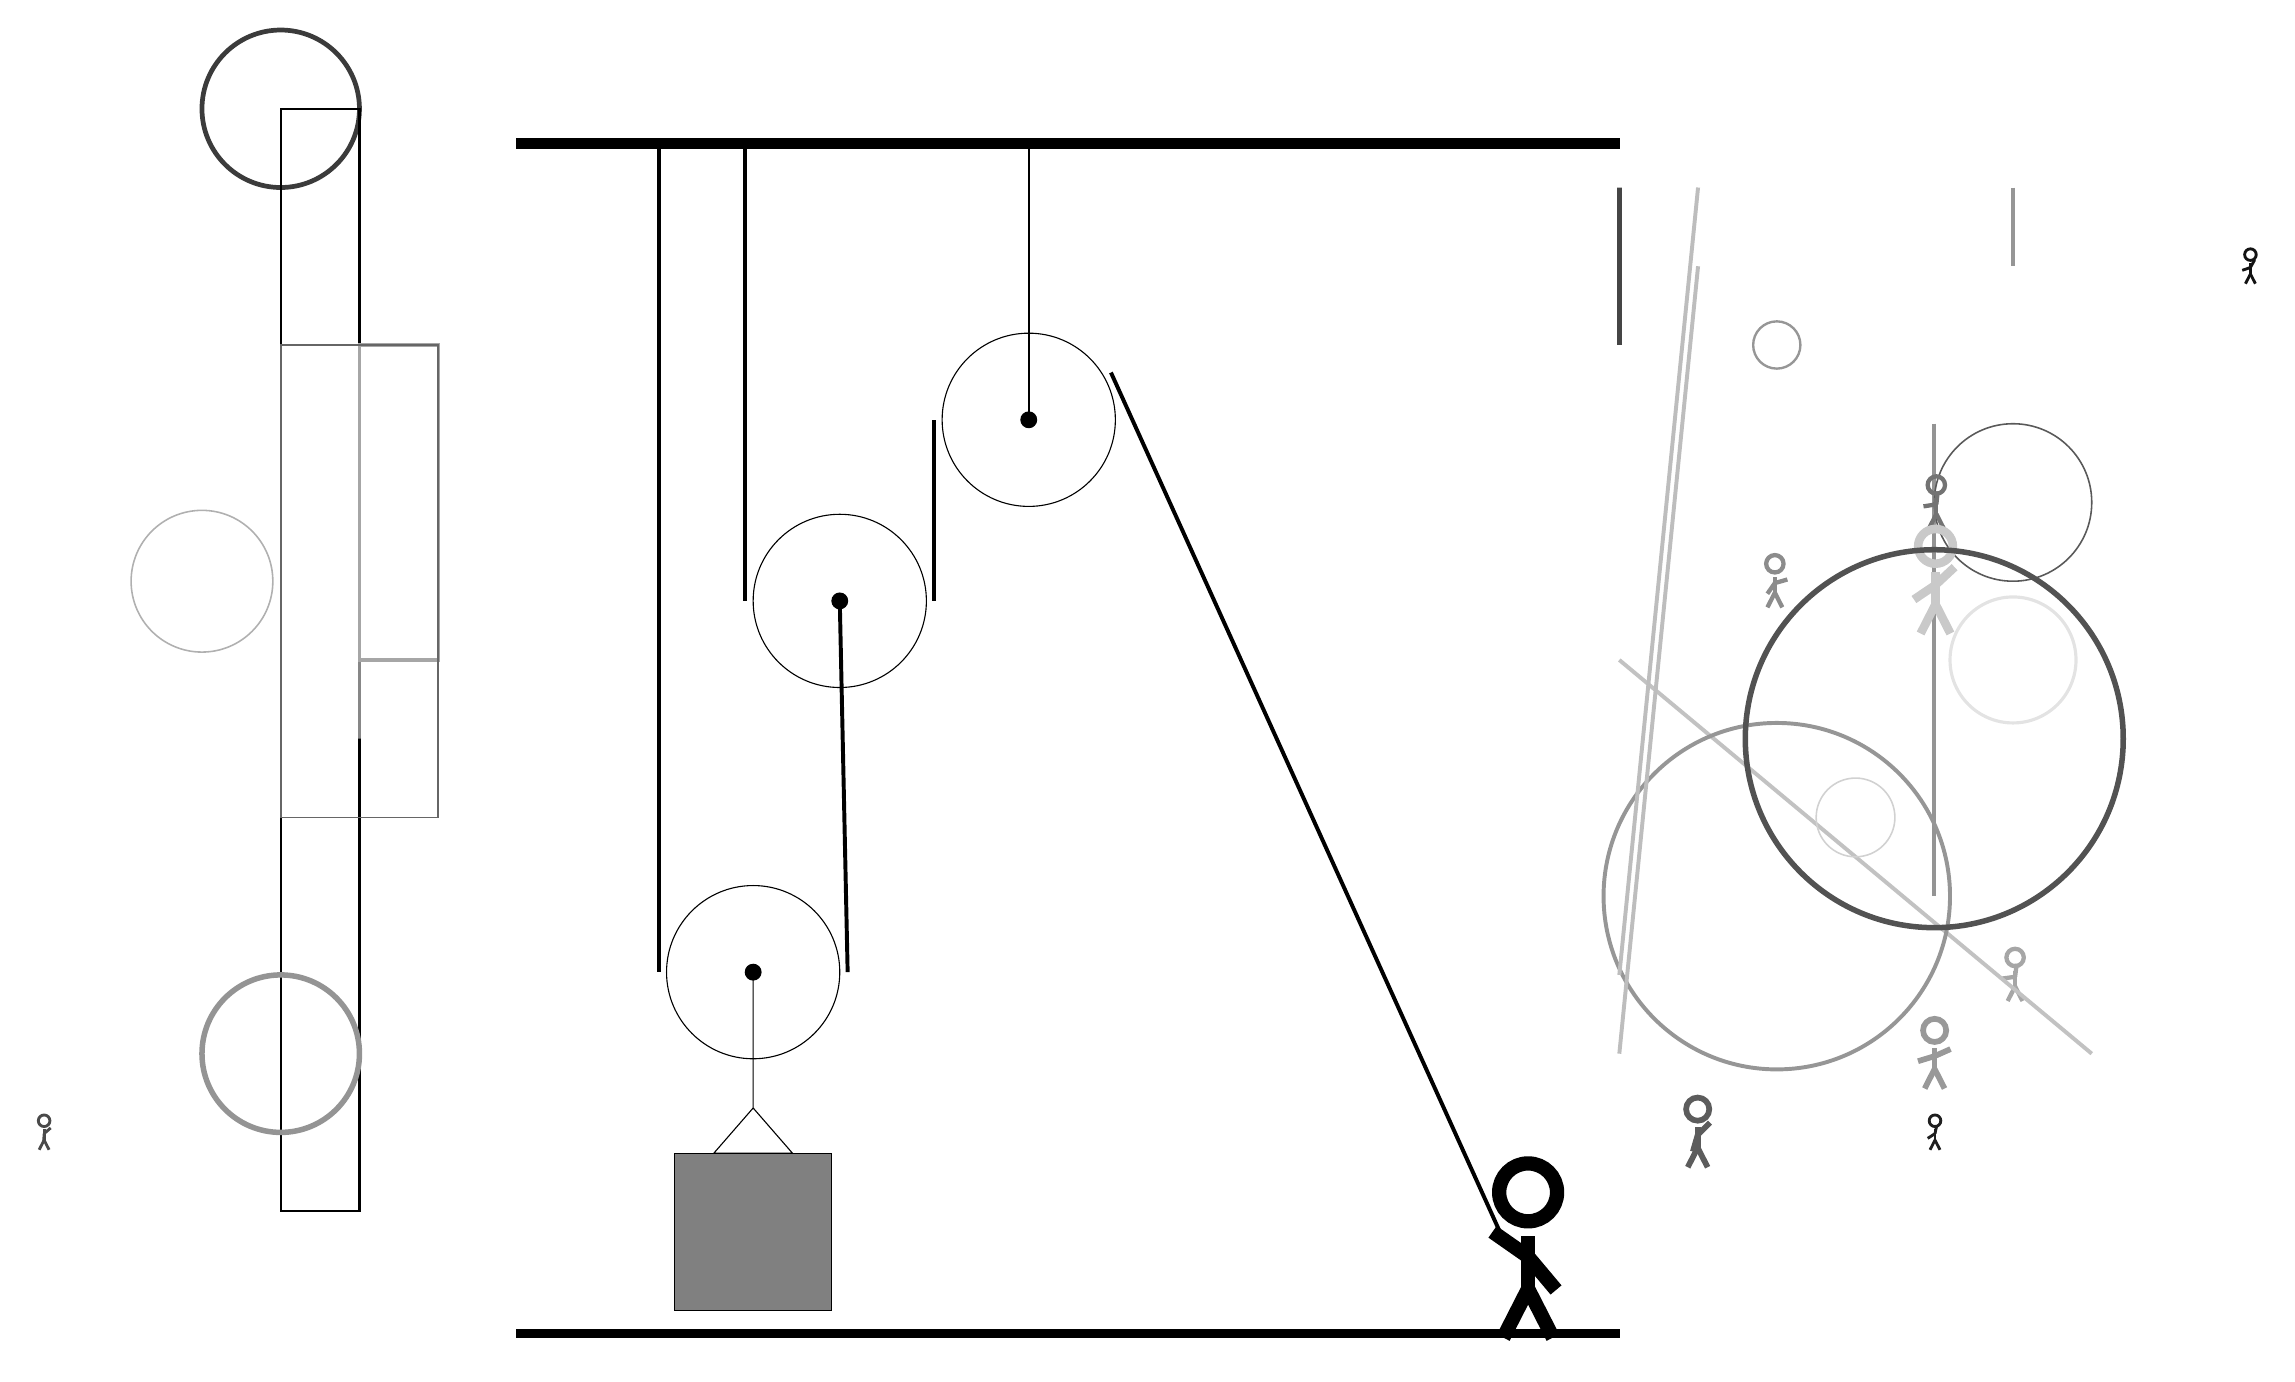
\begin{tikzpicture}
			%%%%% START %%%%%
			
			\draw[fill=black] (-2, 11.5) rectangle (12, 11.625);
			
			\draw (1, 1.035) circle (1.1);
			\draw[fill=black] (1, 1.035) circle (0.1);
			
			\draw (2.1, 5.75) circle (1.1);
			\draw[fill=black] (2.1, 5.75) circle (0.1);
			
			\node[line width=0.7mm, color=black!88] at (16, -1) {\Strichmaxerl[2][33][78]};
			
			\node[line width=0.6mm, color=black!93] at (20, 10) {\Strichmaxerl[2][19][61]};
			\draw [line width=0.3mm, color=black!41](14, 9) circle (0.3);
			\node[line width=0.7mm, color=black!35] at (17, 1) {\Strichmaxerl[3][8][83]};
			\draw [line width=0.4mm, color=black!11](17, 5) circle (0.8);
			\node[line width=0.6mm, color=black!71] at (-8, -1) {\Strichmaxerl[2][87][41]};
			\draw[line width=0.5mm, color=black!42](16, 8) -- (16, 2);
			\draw [line width=0.6mm, color=black!77](-5, 12) circle (1.0);
			\draw[line width=0.6mm, color=black!73] (12, 9) rectangle (12, 11);
			\node[line width=0.2mm, color=black!40] at (16, 0) {\Strichmaxerl[4][17][24]};
			\draw[line width=0.5mm, color=black!24](12, 5) -- (18, 0);
			
			\draw [line width=0.2mm, color=black!31](-6, 6) circle (0.9);
			\draw[line width=0.3mm, color=black!100] (-4, 12) rectangle (-5, -2);
			\draw [line width=0.2mm, color=black!65](17, 7) circle (1.0);
			\draw [line width=0.2mm, color=black!18](15, 3) circle (0.5);
			\node[line width=0.7mm, color=black!55] at (16, 7) {\Strichmaxerl[3][9][84]};
			\draw [line width=0.5mm, color=black!41](14, 2) circle (2.2);
			\draw[line width=0.5mm, color=black!26](13, 10) -- (12, 0);
			\draw[line width=0.3mm, color=black!47] (-4, 6) rectangle (-4, 4);
			
			\node[line width=0.7mm, color=black!21] at (16, 6) {\Strichmaxerl[6][34][43]};
			\node[line width=0.3mm, color=black!45] at (14, 6) {\Strichmaxerl[3][55][16]};
			\draw[line width=0.4mm, color=black!35] (-4, 9) rectangle (-3, 5);
			\draw[line width=0.5mm, color=black!26](13, 11) -- (12, 1);
			\draw[line width=0.5mm, color=black!41](17, 11) -- (17, 10);
			\draw [line width=0.7mm, color=black!68](16, 4) circle (2.4);
			\draw [line width=0.7mm, color=black!42](-5, 0) circle (1.0);
			
			\node[line width=0.2mm, color=black!64] at (13, -1) {\Strichmaxerl[4][74][45]};
			\draw[line width=0.2mm, color=black!60] (-3, 3) rectangle (-5, 9);
			
			\draw (4.5, 8.05) circle (1.1);
			\draw[fill=black] (4.5, 8.05) circle (0.1);
			\draw[thick] (4.5, 8.05) -- (4.5, 11.5);
			
			\draw (1, 1.035) -- (1, -0.69) -- (0.5, -1.265) -- (1.5, -1.265) -- (1, -0.69);
			\draw[fill=black!50] (0, -1.265) rectangle (2, -3.265);
			
			\draw[line width=0.5mm] (-0.2, 11.5) -- (-0.2, 1.035);
			\centerarc[line width=0.5mm](1, 1.035)(180:360:1.2000000000000002);
			\draw[line width=0.5mm](2.2, 1.035) -- (2.1, 5.75);
			\draw[line width=0.5mm] (0.9, 11.5) -- (0.9, 5.75);
			\centerarc[line width=0.5mm](2.1, 5.75)(180:360:1.2000000000000002);
			\draw[line width=0.5mm](3.3, 5.75) -- (3.3, 8.05);
			\centerarc[line width=0.5mm](4.5, 8.05)(30:180:1.2000000000000002);
			\draw[line width=0.5mm] (5.544, 8.65) -- (10.5, -2.3);
			
			\node at (10.8, -2.5) {\Strichmaxerl[10][-35][-50]};
			
			\draw[fill=black] (-2, -3.5) rectangle (12, -3.6);
			
			%%%%% END %%%%%
		\end{tikzpicture}
	\end{figure}	
\end{document}